\documentclass[
  % all of the below options are optional and can be left out
  % course name (default: 2IL50 Data Structures)
  course = {{16-720B Computer Vision}},
  % quartile (default: 3)
  quartile = {{1}},
  % assignment number/name (default: 1)
  assignment = 1-Hough\ Transform,
  % student name (default: Some One)
  name = {{Kangle Deng}},
  % student number, NOT S-number (default: 0123456)
  % studentnumber = {{0123456 ; 0314159}},
  % student email (default: s.one@student.tue.nl)
  email = {{kangled@andrew.cmu.edu}},
  % first exercise number (default: 1)
  firstexercise = 1
]{aga-homework}

\usepackage{url}

\begin{document}
\section{Theory Questions}
\subexercise 
\begin{equation*}
\rho = x\cos{\theta}+y\sin{\theta} = 
\begin{cases}
\sqrt{x^2 + y^2} \sin{(\theta+\arctan\frac{x}{y})}, & y>0,\\
x \sin{(\theta+\frac{\pi}{2})},& y=0,\\
\sqrt{x^2 + y^2} \sin{(\theta+\arctan\frac{x}{y}+\pi)}, & y<0.\\
\end{cases}
\end{equation*}
Therefore, the amplitude $A = \sqrt{x^2 + y^2}$, and
\begin{equation*}
    \text{the phase } \phi = 
    \begin{cases}
\arctan\frac{x}{y}, & y>0,\\
\frac{\pi}{2},& y=0,\\
\arctan\frac{x}{y}+\pi, & y<0.\\
\end{cases}
\end{equation*}

\subexercise
Because the ranges of the slope $m$ and the intercept $c$ are  $(-\infty, +\infty)$, which makes the parameter space really huge, while $\theta \in [0, 2\pi)$, and the range of $\rho$ is determined by the image size.
\begin{equation*}
    m = -\cot{\theta}, \quad c = \frac{\rho}{\sin{\theta}}.
\end{equation*}

\subexercise
$\rho_{max}$ is the maximum distance from the origin to the line, so $\rho_{max} = \sqrt{W^2+H^2}$.

% $\theta$ is the angle from the x-axis to the normal vector of the line, so $\theta \in [0, \pi) \cup (\frac{3\pi}{2}, 2\pi)$.
To make $(\rho, \theta) \rightarrow (m,c)$ a one-to-one mapping, the range of $\theta$ should be $[0, \pi)$, and $\rho$ can be positive or negative. 

\subexercise
From Fig.\ref{fig:Q2.4}, $\rho=0, \theta=\frac{3\pi}{4}$. Therefore, $m=-\cot{\theta}=1, c=\frac{\rho}{\sin{\theta}}=0$.

\begin{figure}[h]
    \centering
    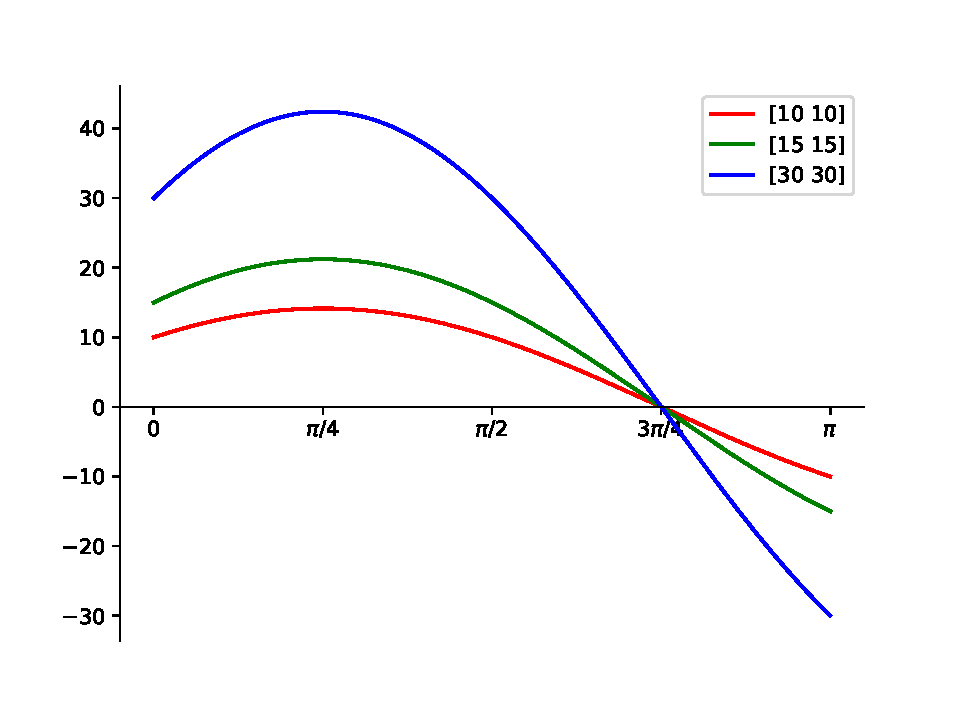
\includegraphics[width = .6\textwidth]{CV/fig/Q4.pdf}
    \caption{Q2.4}
    \label{fig:Q2.4}
\end{figure}

\subexercise
High dimensional Hough Transform should not be much different from the original one, except that the accumulator array is also high dimensional. The steps are similar:
\begin{enumerate}
    \item Define a parameterization of the shape we want to detect. (High dimension means more parameters than 2.)
    \item Quantize the parameter space and create a high-dimensional accumulator array for it.
    \item For each point, vote in the right place in the accumulator array.
    \item Find the local maximum in the accumulator array.
\end{enumerate}

The main steps are similar except that high dimension makes searching for maximum take more time. And also, it will make the accumulator array more sparse, so we can use a count window when searching for the maximum point. 

\section{Resulting Images}
\subsection{Convolution}
I pad the image with `nearest' pixels. Fig.\ref{fig:convolution} is the result images.

\begin{figure}
    \centering
    \subfigure{
        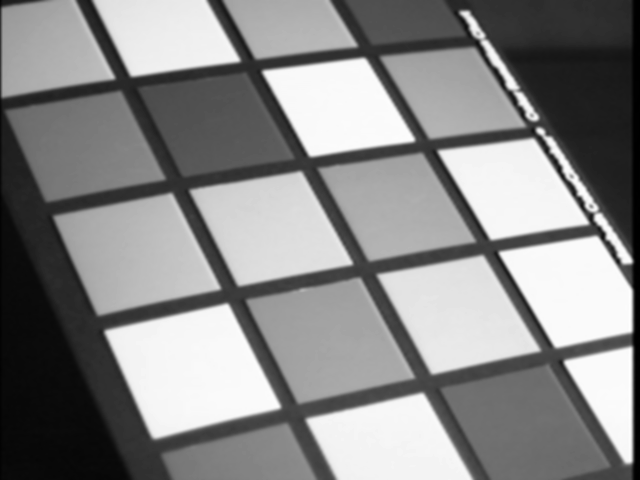
\includegraphics[width=0.48 \textwidth]{CV/fig/results/img01_01Blur.png}
    }
    \subfigure{
        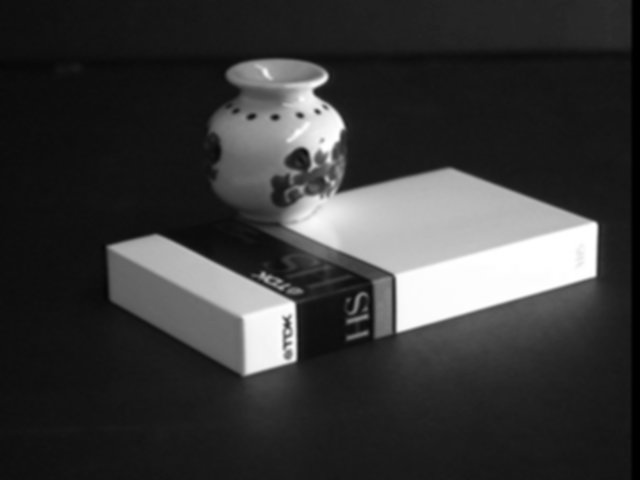
\includegraphics[width=0.48 \textwidth]{CV/fig/results/img02_01Blur.png}
    }
    \subfigure{
        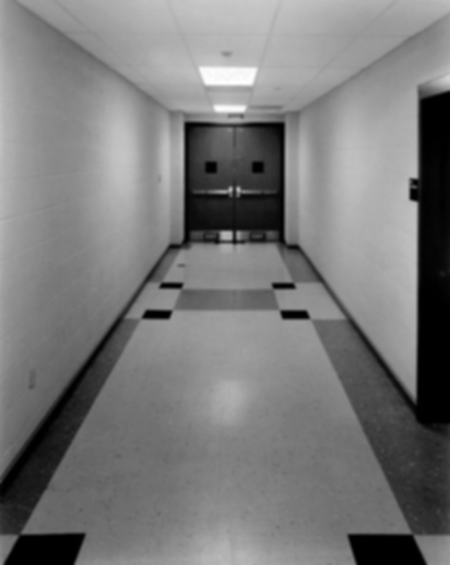
\includegraphics[width=0.33 \textwidth]{CV/fig/results/img03_01Blur.png}
    }
    \subfigure{
        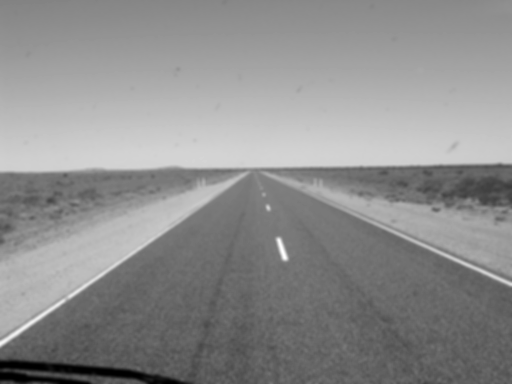
\includegraphics[width=0.55 \textwidth]{CV/fig/results/img04_01Blur.png}
    }
    \subfigure{
        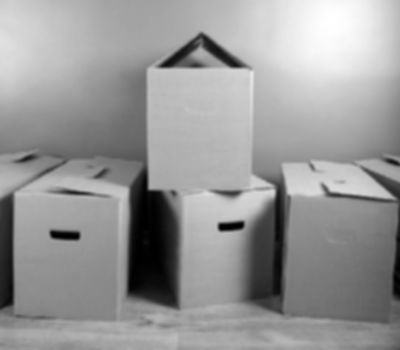
\includegraphics[width=0.3 \textwidth]{CV/fig/results/img05_01Blur.png}
    }
    \subfigure{
        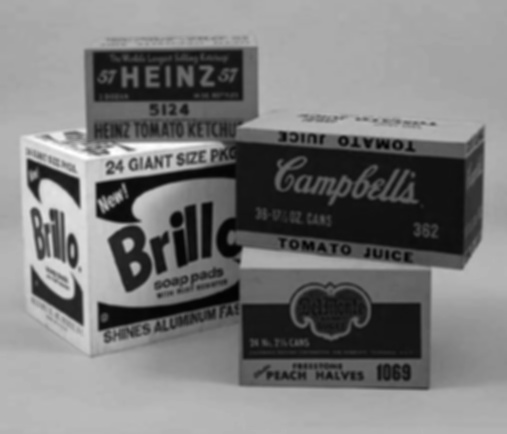
\includegraphics[width=0.3 \textwidth]{CV/fig/results/img06_01Blur.png}
    }
    \subfigure{
        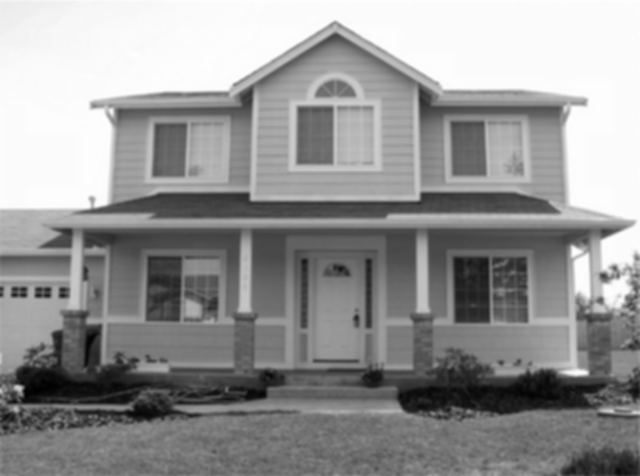
\includegraphics[width=0.35 \textwidth]{CV/fig/results/img07_01Blur.png}
    }
    \subfigure{
        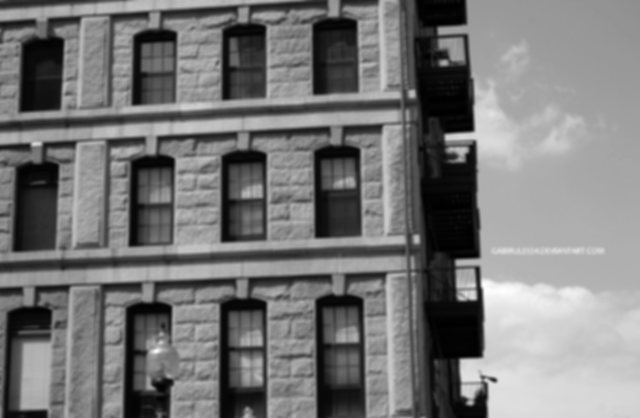
\includegraphics[width=0.42 \textwidth]{CV/fig/results/img08_01Blur.png}
    }
    \subfigure{
        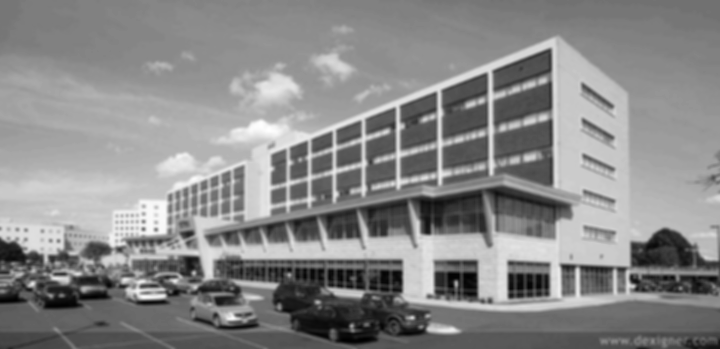
\includegraphics[width=0.54 \textwidth]{CV/fig/results/img09_01Blur.png}
    }

    \caption{Results of 2.1 Convolution}
    \label{fig:convolution}
\end{figure}

\subsection{Convolution with One $for$ Loop}
If we flip the convolution filter and flatten it as a vector, the operation of multiplying filter elements with corresponding pixels in the image and then summing up can be regarded as a dot product between 2 vectors. So the main idea is to represent the convolution as a matrix multiplication operation between a matrix $A$ and a vector $v$. Let $h$ and $w$ denote the size of the image, and $fh$ and $fw$ denote the size of the filter.

$A$ has the size of $(h\times w) \times (fh \times fw)$. Each column of $A$ is the corresponding pixels that should be involved in each step of convolution. $v$, with the length of $(fh \times fw)$, is the flattened flipped filter. 

The calculation of matrix multiplication is fully vectorized and involves no $for$ loop. However, I use one $for$ loop when constructing $A$.

\subsection{Edge Detection}
The size of the Gaussian filter is set as $hsize = 2 \cdot ceil(3\cdot \sigma) + 1$. $Io$ is set to be $0$ if both $Ix$ and $Iy$ are $0$. The function returns $Io$ as a quantized matrix of 4 values - $0^{\circ}, 45^{\circ}, 90^{\circ}$ and $135^{\circ}$. Fig. \ref{fig:edge} is the result images.


\begin{figure}
    \centering
    \subfigure{
        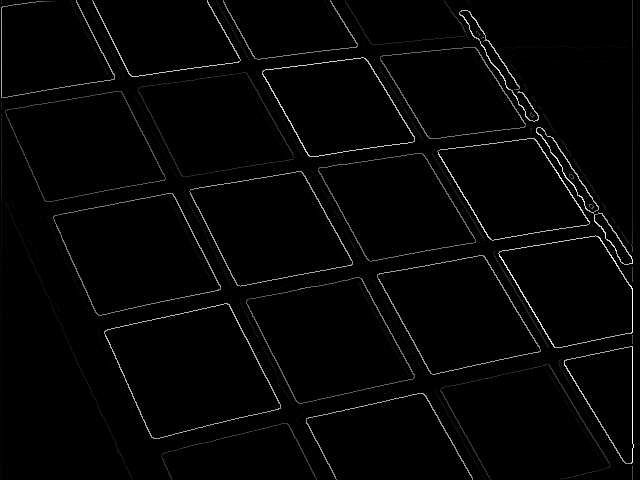
\includegraphics[width=0.48 \textwidth]{CV/fig/results/img01_03edge.png}
    }
    \subfigure{
        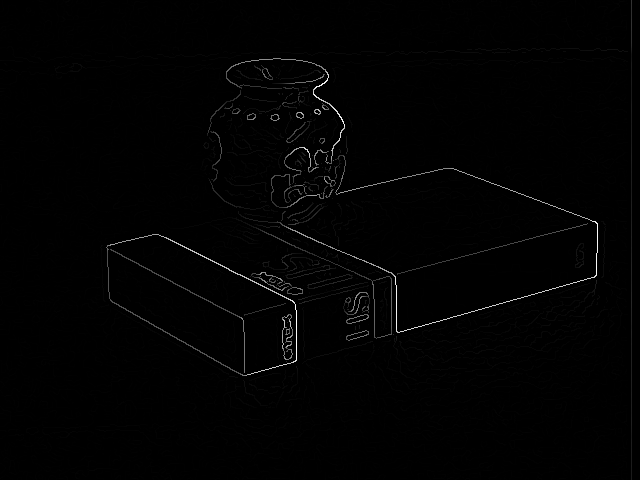
\includegraphics[width=0.48 \textwidth]{CV/fig/results/img02_03edge.png}
    }
    \subfigure{
        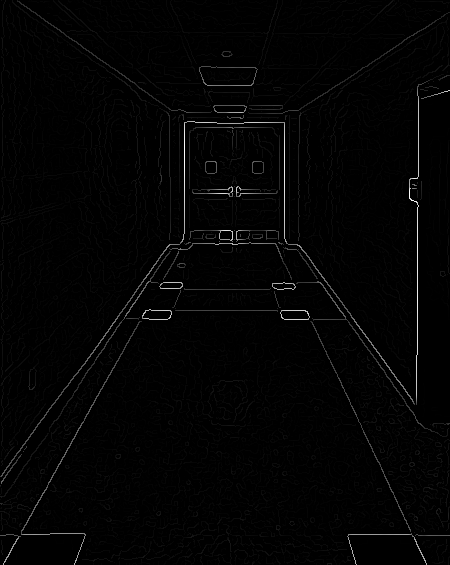
\includegraphics[width=0.33 \textwidth]{CV/fig/results/img03_03edge.png}
    }
    \subfigure{
        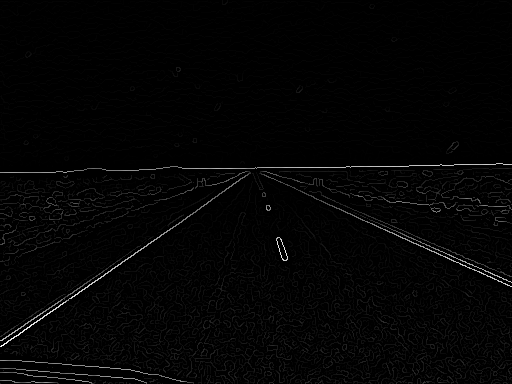
\includegraphics[width=0.55 \textwidth]{CV/fig/results/img04_03edge.png}
    }
    \subfigure{
        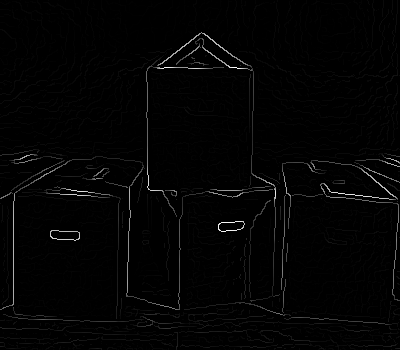
\includegraphics[width=0.3 \textwidth]{CV/fig/results/img05_03edge.png}
    }
    \subfigure{
        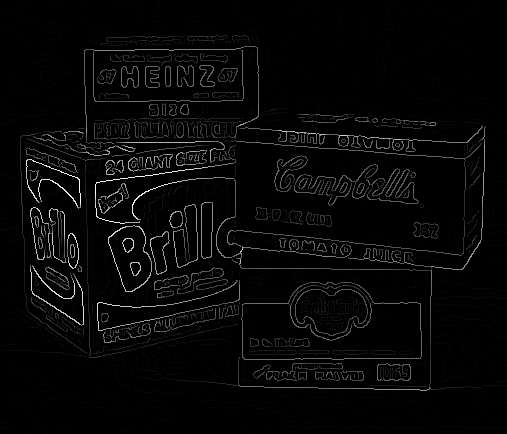
\includegraphics[width=0.3 \textwidth]{CV/fig/results/img06_03edge.png}
    }
    \subfigure{
        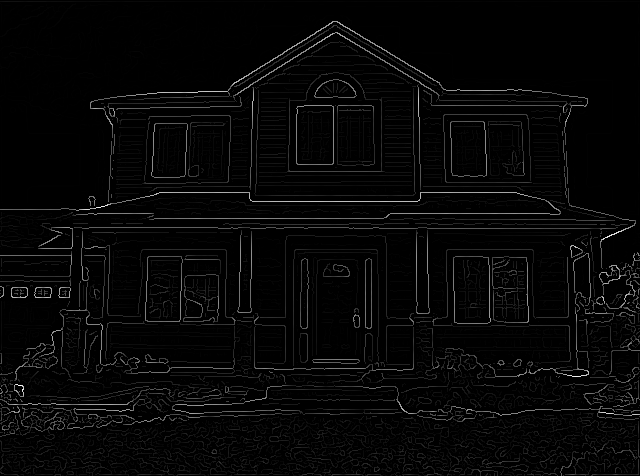
\includegraphics[width=0.35 \textwidth]{CV/fig/results/img07_03edge.png}
    }
    \subfigure{
        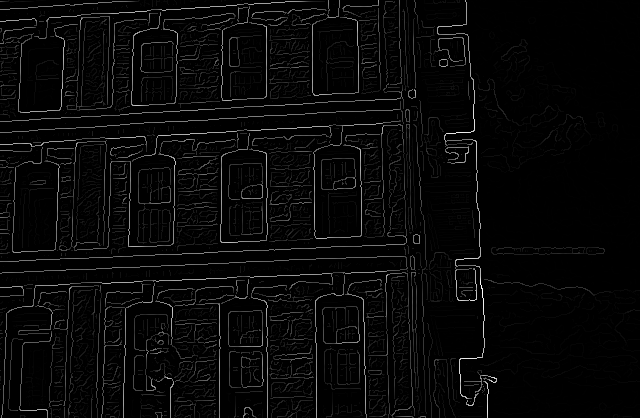
\includegraphics[width=0.42 \textwidth]{CV/fig/results/img08_03edge.png}
    }
    \subfigure{
        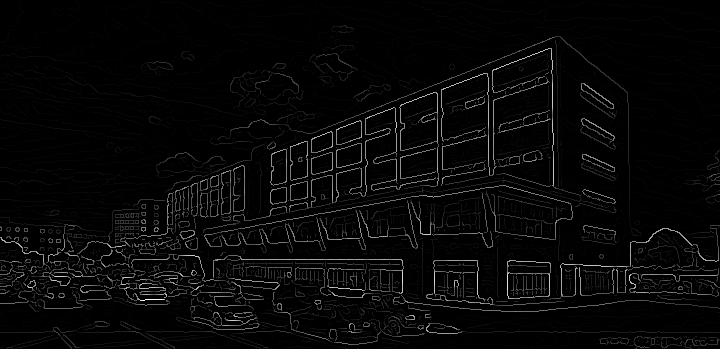
\includegraphics[width=0.54 \textwidth]{CV/fig/results/img09_03edge.png}
    }

    \caption{Results of 2.3 Edge Detection}
    \label{fig:edge}
\end{figure}

\begin{figure}
    \centering
    \subfigure{
        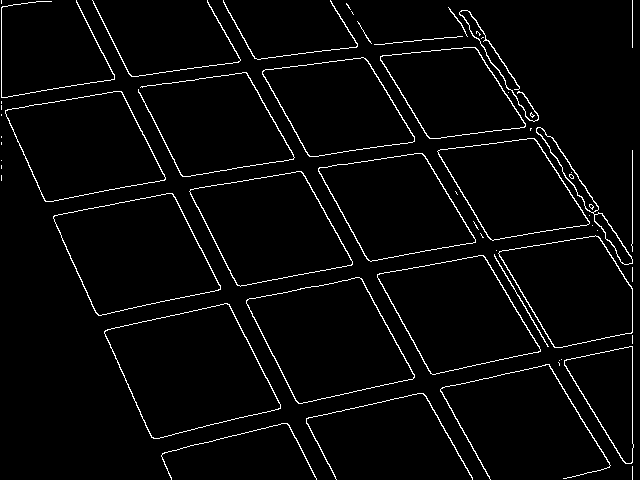
\includegraphics[width=0.48 \textwidth]{CV/fig/results/img01_04threshold.png}
    }
    \subfigure{
        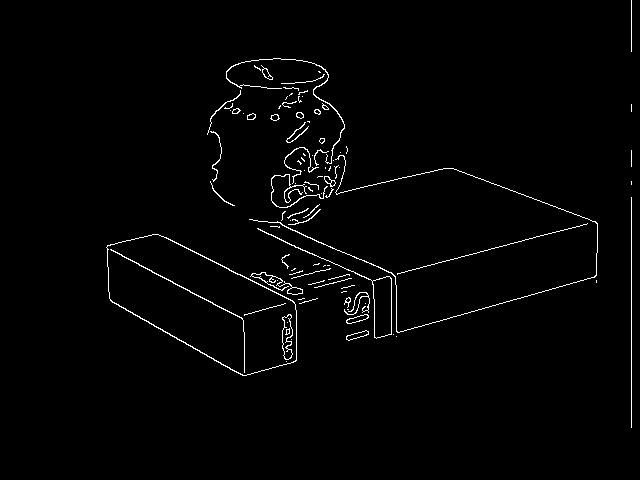
\includegraphics[width=0.48 \textwidth]{CV/fig/results/img02_04threshold.png}
    }
    \subfigure{
        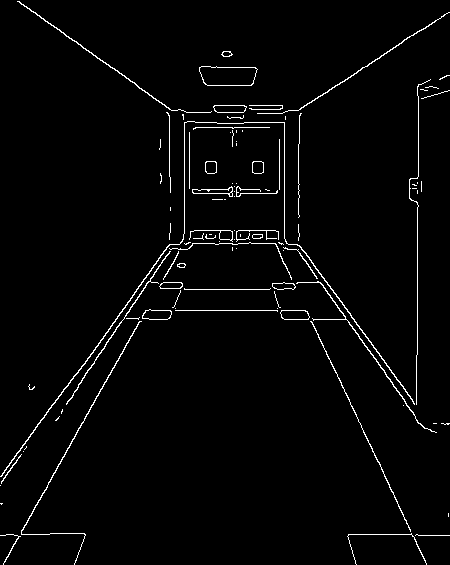
\includegraphics[width=0.33 \textwidth]{CV/fig/results/img03_04threshold.png}
    }
    \subfigure{
        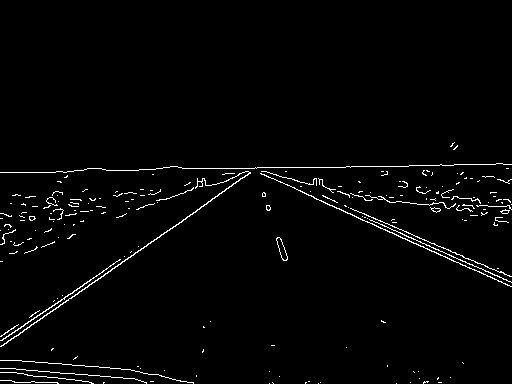
\includegraphics[width=0.55 \textwidth]{CV/fig/results/img04_04threshold.png}
    }
    \subfigure{
        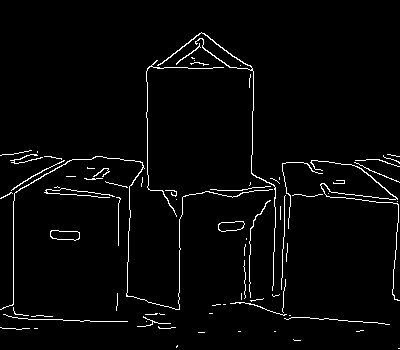
\includegraphics[width=0.3 \textwidth]{CV/fig/results/img05_04threshold.png}
    }
    \subfigure{
        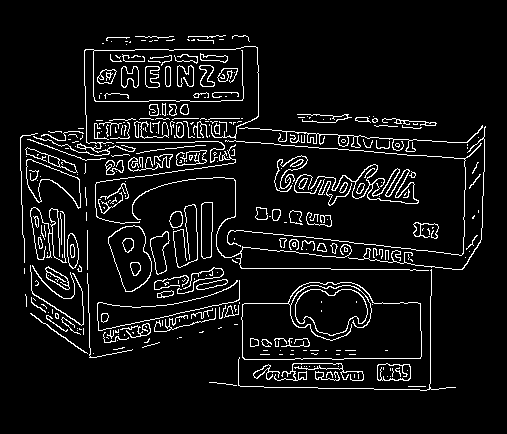
\includegraphics[width=0.3 \textwidth]{CV/fig/results/img06_04threshold.png}
    }
    \subfigure{
        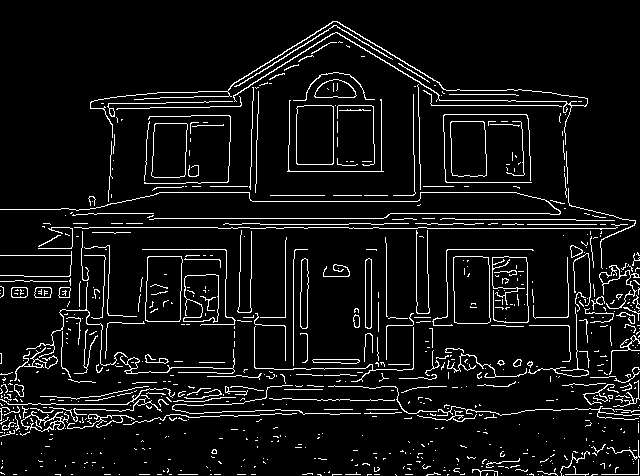
\includegraphics[width=0.35 \textwidth]{CV/fig/results/img07_04threshold.png}
    }
    \subfigure{
        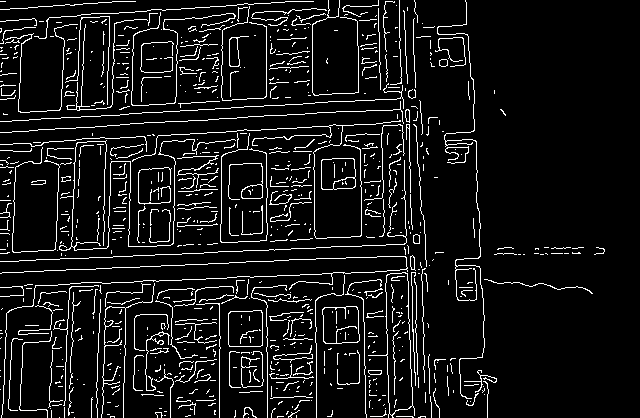
\includegraphics[width=0.42 \textwidth]{CV/fig/results/img08_04threshold.png}
    }
    \subfigure{
        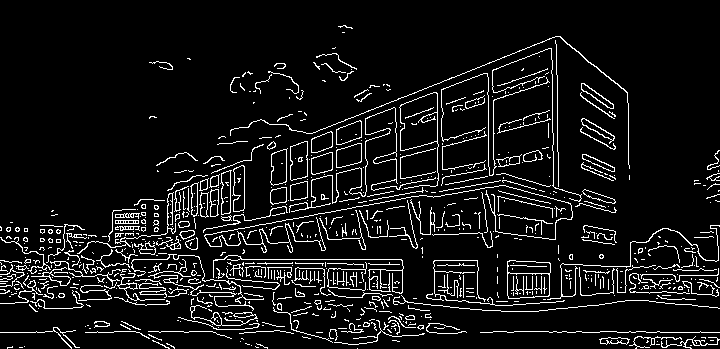
\includegraphics[width=0.54 \textwidth]{CV/fig/results/img09_04threshold.png}
    }

    \caption{Results of Thresholded Edge Image}
    \label{fig:threshold}
\end{figure}

\subsection{Hough Transform}
Fig. \ref{fig:hough} is the result images.


\begin{figure}
    \centering
    \subfigure{
        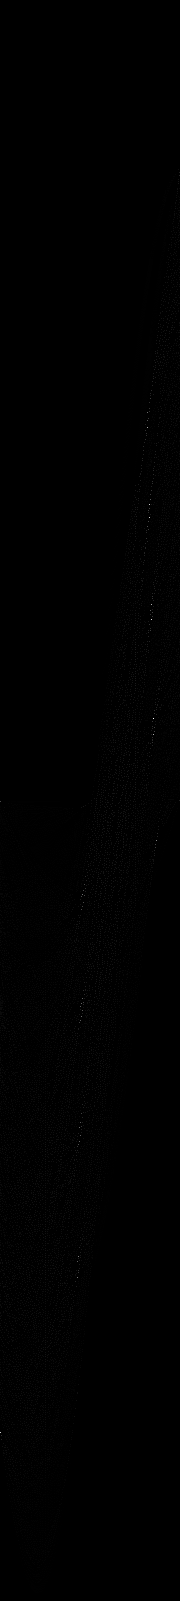
\includegraphics[width=0.08 \textwidth]{CV/fig/results/img01_05Hough.png}
    }
    \subfigure{
        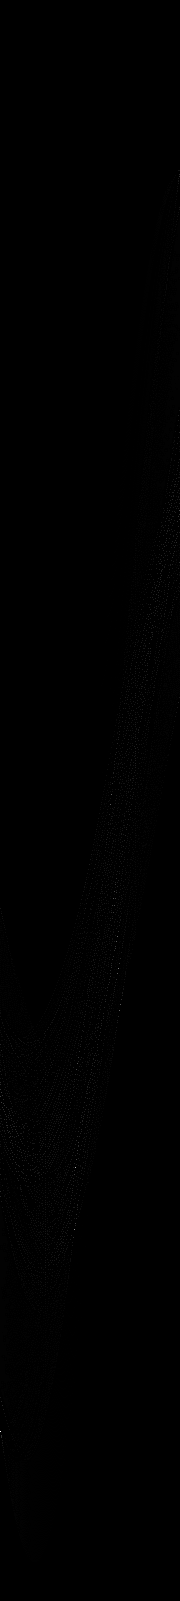
\includegraphics[width=0.08 \textwidth]{CV/fig/results/img02_05Hough.png}
    }
    \subfigure{
        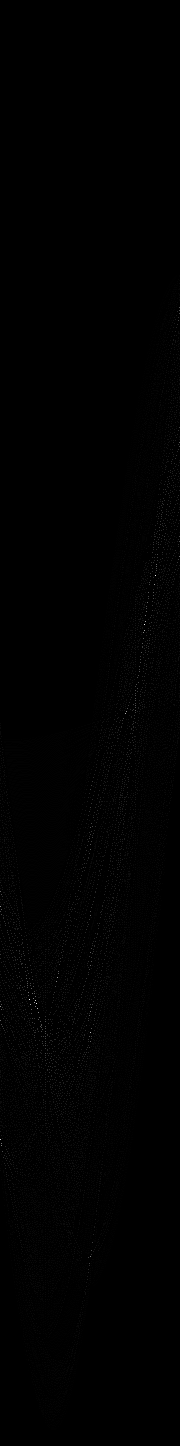
\includegraphics[width=0.08 \textwidth]{CV/fig/results/img03_05Hough.png}
    }
    \subfigure{
        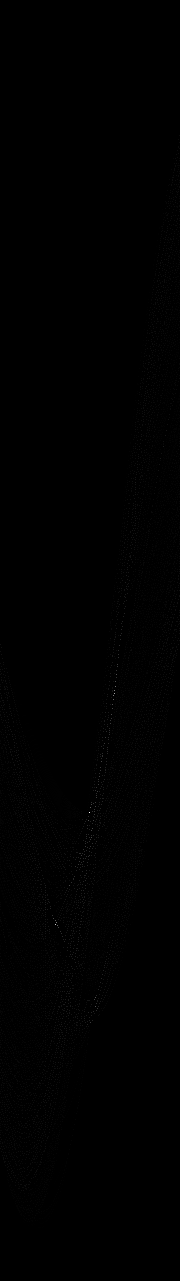
\includegraphics[width=0.08 \textwidth]{CV/fig/results/img04_05Hough.png}
    }
    \subfigure{
        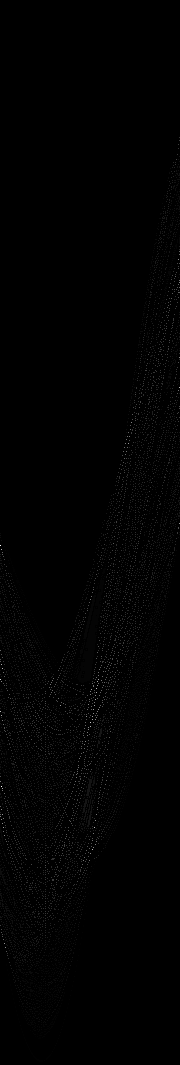
\includegraphics[width=0.08 \textwidth]{CV/fig/results/img05_05Hough.png}
    }
    \subfigure{
        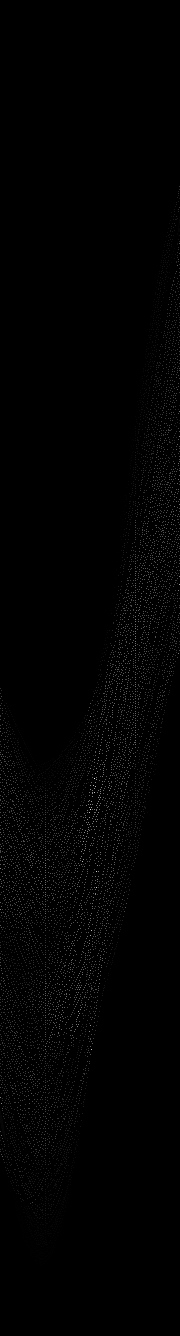
\includegraphics[width=0.08 \textwidth]{CV/fig/results/img06_05Hough.png}
    }
    \subfigure{
        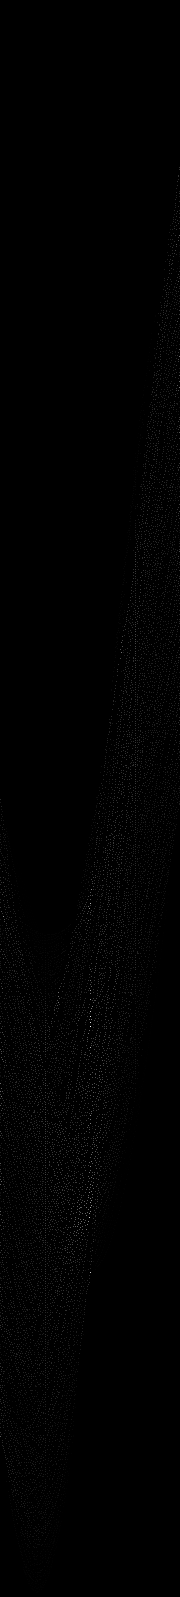
\includegraphics[width=0.08 \textwidth]{CV/fig/results/img07_05Hough.png}
    }
    \subfigure{
        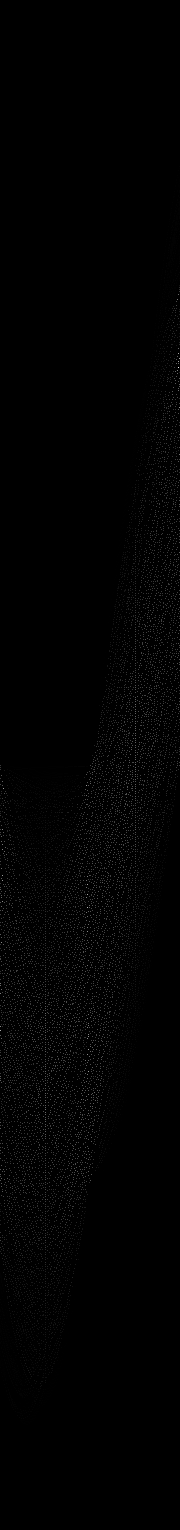
\includegraphics[width=0.1 \textwidth]{CV/fig/results/img08_05Hough.png}
    }
    \subfigure{
        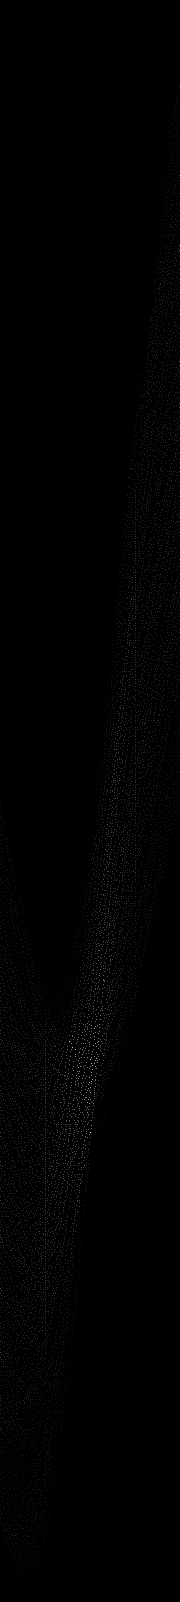
\includegraphics[width=0.1 \textwidth]{CV/fig/results/img09_05Hough.png}
    }

    \caption{Results of 2.4 Hough Transform}
    \label{fig:hough}
\end{figure}

\subsection{Finding Lines}
When implementing a function of finding top $n$ values in a 2d matrix, I find the information at \url{https://includestdio.com/1557.html} useful.

To get rid of close high values in the accumulator matrix, I implement non maximal suppression with a variable window size. See Section 4 Table 2 for experiments on different window sizes of NMS.

\subsection{Fitting Line Segments for Visualization}
For each line found in last step, I first specify those points that are valid within the image size. For each point, check if there is any edge around in $ThrImEdge$, the result of Q3.3. This is implemented by first convolving $ThrImEdge$ with a gaussian filter, and then checking whether the pixel on that position is greater than zero. Finally, I change those points to green to visulize the line segments. Note that all of the operations above are implemented in a vectorized way, so it does not cost much time. Fig.\ref{fig:final} is the result images.

\begin{figure}
    \centering
    \subfigure{
        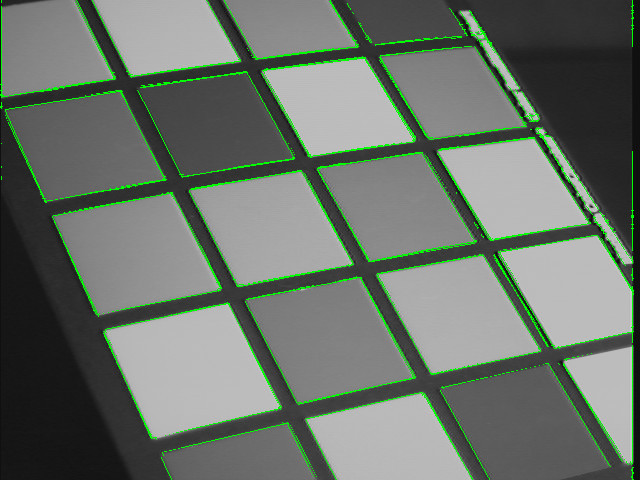
\includegraphics[width=0.48 \textwidth]{CV/fig/results/img01_06Final.png}
    }
    \subfigure{
        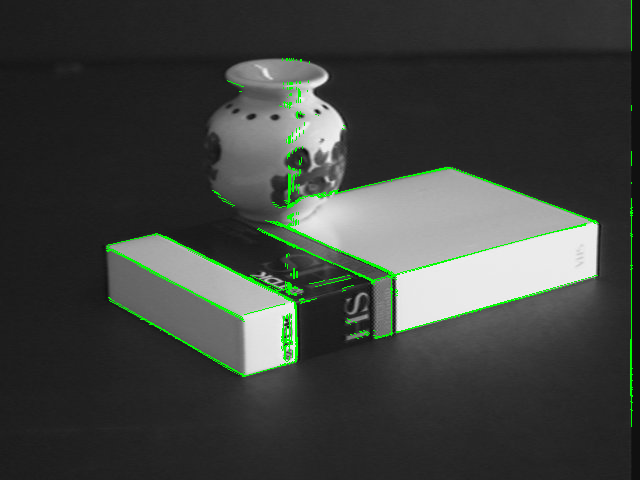
\includegraphics[width=0.48 \textwidth]{CV/fig/results/img02_06Final.png}
    }
    \subfigure{
        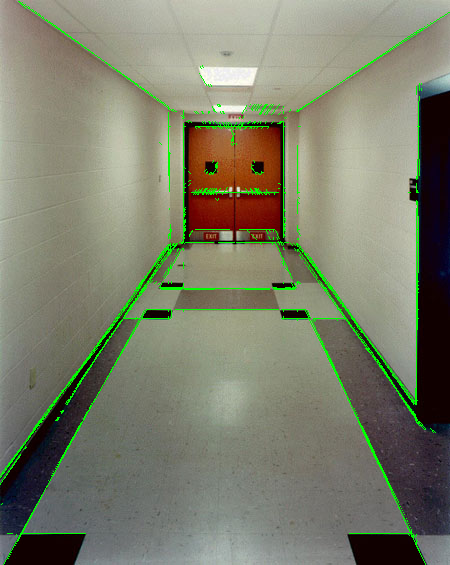
\includegraphics[width=0.33 \textwidth]{CV/fig/results/img03_06Final.png}
    }
    \subfigure{
        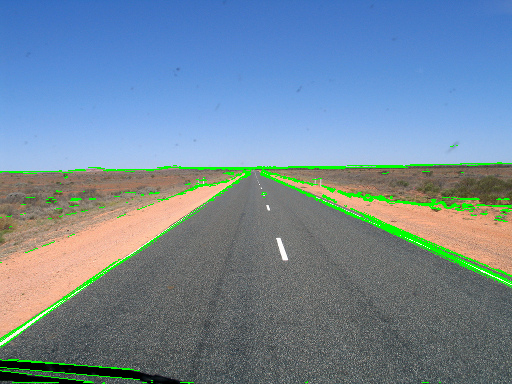
\includegraphics[width=0.55 \textwidth]{CV/fig/results/img04_06Final.png}
    }
    \subfigure{
        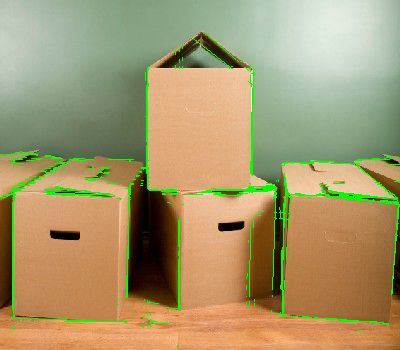
\includegraphics[width=0.3 \textwidth]{CV/fig/results/img05_06Final.png}
    }
    \subfigure{
        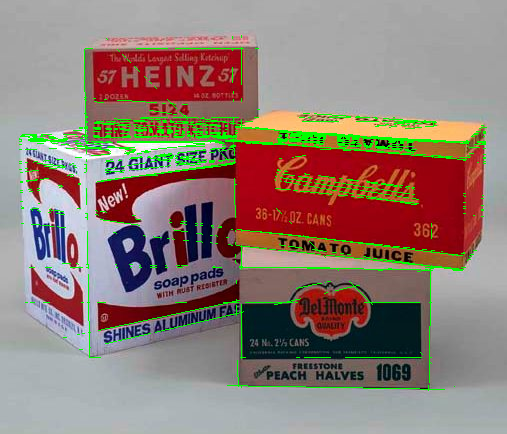
\includegraphics[width=0.3 \textwidth]{CV/fig/results/img06_06Final.png}
    }
    \subfigure{
        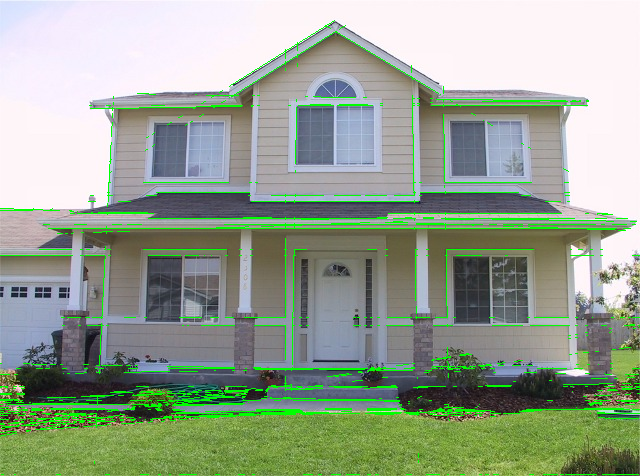
\includegraphics[width=0.35 \textwidth]{CV/fig/results/img07_06Final.png}
    }
    \subfigure{
        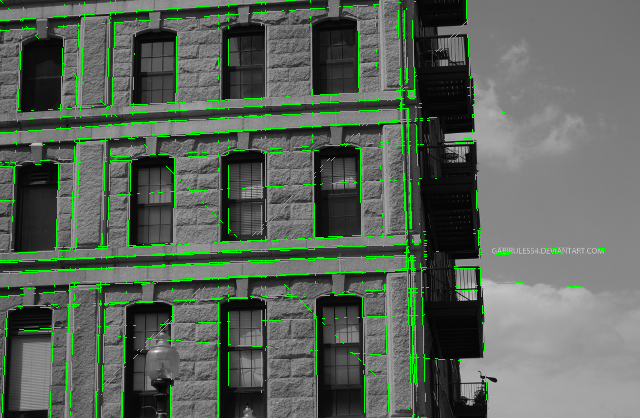
\includegraphics[width=0.42 \textwidth]{CV/fig/results/img08_06Final.png}
    }
    \subfigure{
        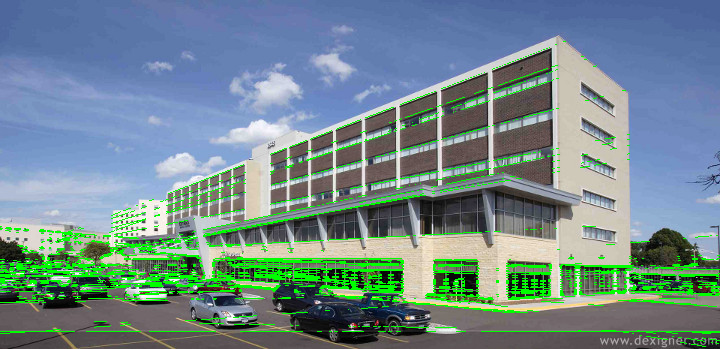
\includegraphics[width=0.54 \textwidth]{CV/fig/results/img09_06Final.png}
    }

    \caption{Results of 2.6 Fitting Line Segments}
    \label{fig:final}
\end{figure}

\section{Discussions}
Clearly, a single set of parameters cannot work equally well on all the images. In Fig. \ref{fig:final}, my code works better on Img01, Img03, Img04, and Img08 than the rest of test images. Those images only contain simple line structure, and does not contain complex curves such as words in Img06, patterns on the vase in Img02, and messy small objects in Img07 and Img09. In those difficult images, those noises, which are not expected to be detected as line segments, interfere with the detection of useful lines. In this sense, an optimal set of parameters for one image is one that filters away noisy information but keeps valuable information detected.

Although finding optimal parameters for one test image needs a lot of human effort, there exist some `general' guidelines from my experiments:

\begin{itemize}
    \item If there exist a lot of messy small objects in the image (E.g. bushes in Img07, cars in Img09) and one just want to detect the `dominant' lines from it, one should use a larger gaussian filter (also with a larger $\sigma$) as well as a larger edge magnitude threshold, so as to filter away those unimportant but messy line segments. (See Table \ref{tab:thresh_and_sigma}.)
    \item If there are a lot of close lines in the result, one possible solution is to increase the resolution of $\rho$ and $\theta$. However, this will somehow lead to the inaccuracy in finding lines. A more reasonable solution is to use a larger window in the non maximal suppression of finding lines - that is to compare to not only 1-step neighbours but also multi-step ones in the accumulator. (See Table \ref{tab:NMS})
\end{itemize}

\begin{table}
  \begin{center}
    \begin{tabular}{lccc}
      \toprule
      \textbf{$\sigma$ $\backslash$ Thresh} & $\text{Thresh} = 1$ & $\text{Thresh} = 5$ & $\text{Thresh} = 10$\\
      \midrule
      $\sigma=1.5$ & 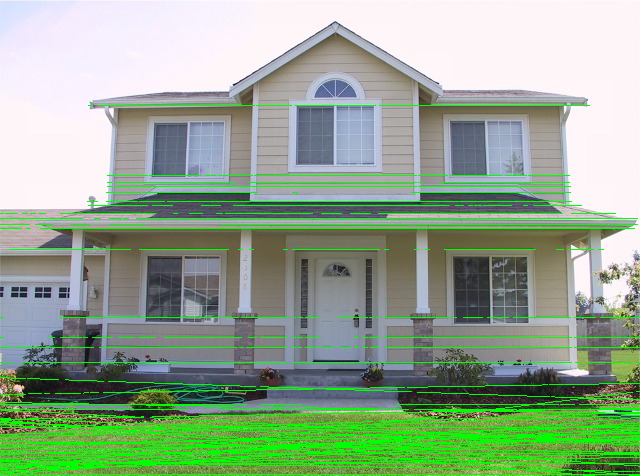
\includegraphics[width=0.25\textwidth]{CV/fig/thresh&sigma/thresh1.png} & 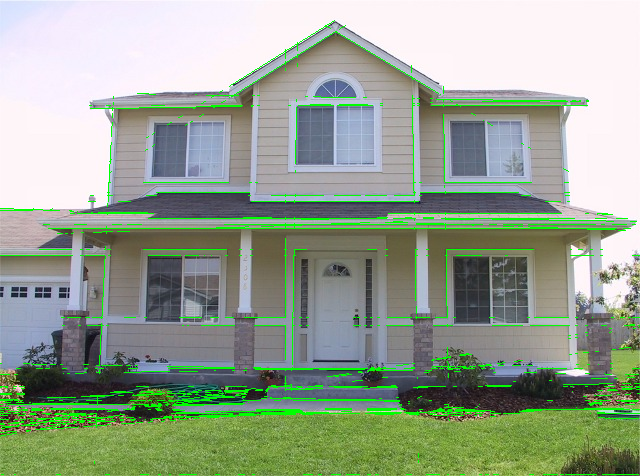
\includegraphics[width=0.25\textwidth]{CV/fig/results/img07_06Final.png} & 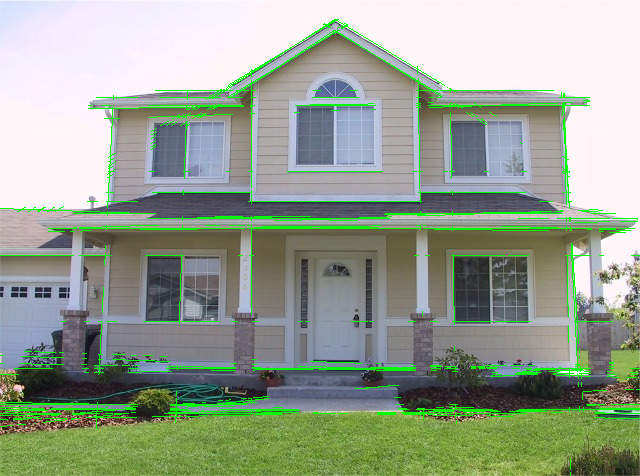
\includegraphics[width=0.25\textwidth]{CV/fig/thresh&sigma/thresh10.png}  \\
      $\sigma=2$ &  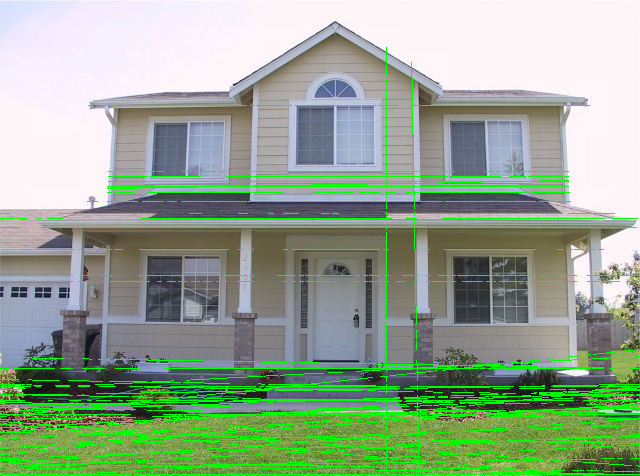
\includegraphics[width=0.25\textwidth]{CV/fig/thresh&sigma/thresh1sigma2.png} & \includegraphics[width=0.25\textwidth]{CV/fig/thresh&sigma/sigma2.png} & \includegraphics[width=0.25\textwidth]{CV/fig/thresh&sigma/thresh10sigma2.png}  \\
      $\sigma=3$ & \includegraphics[width=0.25\textwidth]{CV/fig/thresh&sigma/thresh1sigma3.png} & \includegraphics[width=0.25\textwidth]{CV/fig/thresh&sigma/sigma3.png} & \includegraphics[width=0.25\textwidth]{CV/fig/thresh&sigma/thresh10sigma3.png}  \\
      \bottomrule
    \end{tabular}
  \end{center}
\caption{\textbf{Effect of Gaussian $\sigma$ and Edge Magnitude Threshold.} This experiment selects different values of $\sigma$ and edge threshold to see their effect in detecting lines. The Gaussian kernel size is always set to be $2\times ceil(\sigma) + 1$. There are a lot of bushes containing messy edges, instead of which one would expect to detect those dominant lines of the house. When both Thresh and $\sigma$ are small values (top-left), the detector cannot get rid of the noisy edges, and they prevent the dominant lines from being detected. By either increasing Thresh or $\sigma$, those noises are removed and dominant lines become detected. However, too large $\sigma$ values and Thresh would filter away not only those noises but also useful information (bottom-right).} 
  \label{tab:thresh_and_sigma}
\end{table}

\begin{table}
  \begin{center}
    \begin{tabular}{lcc}
      \toprule
      \textbf{NMS} & window size = 1 & window size = 5 \\
      \midrule
& \includegraphics[width=0.45\textwidth]{CV/fig/NMS/NMS1.png} & \includegraphics[width=0.45\textwidth]{CV/fig/NMS/NMS5.png}  \\
    \end{tabular}
  \end{center}
\caption{\textbf{Effect of NMS Window size.} This experiment selects different sizes of windows when implementing Non maximal suppression on accumulator matrix of Hough Transform. When window size = 1 (left), the visualized lines are `thick' as there are a bunch of close lines clustering. When increasing window size to 5 (right), some lines are thinned as close lines are selected only once through NMS.} 
  \label{tab:NMS}
\end{table}


\end{document}
